\documentclass{article}

\usepackage[T1]{fontenc}
\usepackage[utf8]{inputenc}
\usepackage{float}
\usepackage[french]{babel}
\usepackage[margin=.8in]{geometry}
\usepackage{amssymb}
\usepackage{amsmath}  
\usepackage{mathtools}
\usepackage{listings}
\usepackage{graphicx}
\usepackage[hidelinks]{hyperref}

\begin{document}
    
    \title{Conception et réalisation d'un processeur 8 bits}
    \author{Nathan Soufflet}

    \maketitle
    \pagenumbering{gobble}
    \newpage

    \section{Introduction}

    \paragraph{}
    Ce projet consiste en la conception puis réalisation d'un ordinateur Turing-complet à partir de
    composants discrets élémentaires ainsi que l'ensemble des composantes logicielles permettant son
    utilisation pratique. L'objectif principal est la visualisation et compréhension profonde des
    différentes opérations et couches impliquées dans l'éxécution d'un programme ecrit dans un langage
    haut niveau.

    \section{Partie matérielle}

    \subsection{Organisation en modules}

    \paragraph{}
    Le processeur suit une architecture de von Neumann avec un bus de données 8 bits et un bus d'adresse 16 bits.
    Il est structuré en 9 modules distincts réalisant chacun une fonction très simple 
    contrôlable à l'aide de microcodes, cette approche possède de nombreux avantages : \\
    \begin{itemize}
    \item Segmentation du travail à fournir
    \item Possibilité de tester chaque fonction séparément
    \item Possibilité de faire évoluer chaque module individuellement
    \item Feedback rapide durant la conception
    \end{itemize}
    
    \paragraph{}
    Il se pose toutefois un problème : Comment connecter chaque module aux bus et comment faire en sorte 
    que le module de contrôle ait accès à tous les modules ?
    \paragraph{}
    En effet, du fait de la géometrie rectangulaire
    des modules, chacun d'entre eux ne peut accéder au maximum qu'aux quatre modules connexes.
    Une solution serait alors de faire passer des connexions en-dessous ou au-dessus de certains
    d'entre-eux avec des câbles. Ce n'est cependant pas très élégant et peut entraîner des erreurs
    de branchement.
    Une autre solution a été choisie : les modules se chargeront, en plus de remplir leur fonction,
    de propager des signaux aux modules connexes.)

    \begin{figure}[ht!]
        \label{fig_reg_module}
        \centering
        \includegraphics[width=0.5\textwidth]{figures/Module.png}
        \caption{Propagation du signal d'horloge et du bus de données d'un module de registre}
    \end{figure}

    Une étude sera alors menée sur la disposition optimale des modules permettant de minimiser le nombre
    de signaux à propager ainsi que leur distance.

    \newpage


    \subsection{Architecture}
    \begin{figure}[ht!]
        \label{fig_architecture}
        \centering
        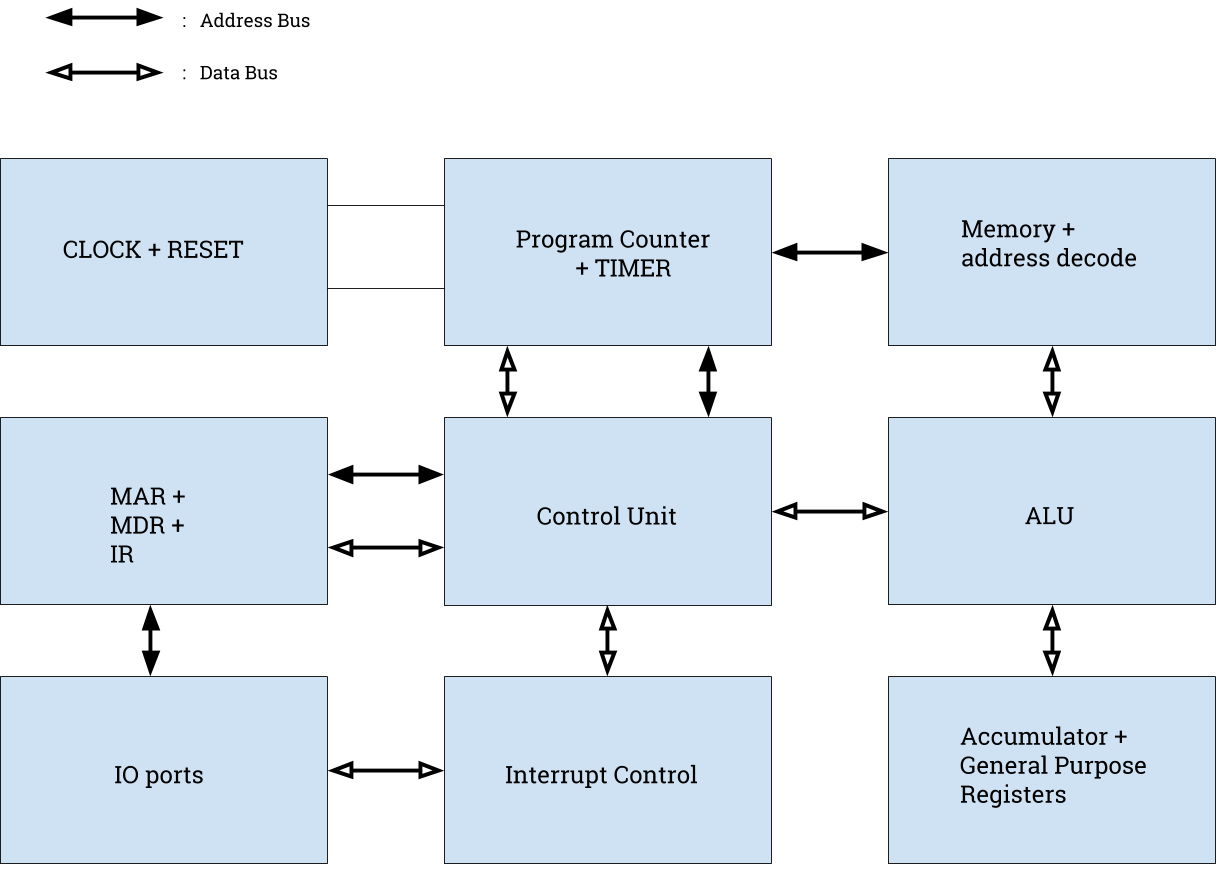
\includegraphics[width=\textwidth]{figures/Architecture.png}
        \caption{Organisation possible des modules}
    \end{figure}

    \subsubsection{CLOCK + RESET}
    \paragraph{}
    Ce module s'occupe de la génération d'un signal carré périodique permettant de synchroniser les 
    opérations des différents modules entre-eux. 
    Il dispose de trois modes d'opération : \\
    \begin{itemize}
        \item Lent : Permet de faire varier la fréquence entre 0.8 et 400Hz            
        \item Rapide : Permet de faire varier la fréquence entre 1kHz et 1.6MHz            
        \item Manuel : Permet de contrôler manuellement l'horloge (mode pas à pas)            
    \end{itemize}
    
    \paragraph{}
    La seconde fonction de ce module est de réinitialiser le processeur pendant la première demi-seconde
    après allumage (de sorte à ce que la tension se stabilise à 5V garantissant le bon fonctionnement des modules)
    et à chaque appui d'un bouton dédié.


    \subsubsection{Program Counter + Timer}
    \paragraph{}
    Ce module contient deux registres 16 bits:

    \begin{itemize}
        \item Program Counter : Contient l'adresse de la prochaine instruction à décoder
        \item Timer : Contient le nombre de cycles écoulés depuis l'allumage (modulo $2^{16}$)      
    \end{itemize}  

    \newpage

    \subsubsection{Memory + Address decode}
    \paragraph{}
    Ce module contient la ROM (32k premiers octets : mémoire contenant les instructions) et la RAM
    (32k derniers octets : mémoire contenant les données)
    ainsi que la logique de décodage d'adresse permettant de selectionner la banque mémoire dans laquelle lire
    ou écrire des données.
    

    \subsubsection{MAR + MDR + IR}
    \paragraph{}
    Ce module contient trois registres:

    \begin{itemize}
        \item Instruction Register (IR - 8 bits) : Contient la prochaine instruction à exécuter 
        \item Memory Address Register (MAR - 16 bits) : Contient l'adresse selectionnée dans le module mémoire 
        \item Memory Data Register (MAR - 16 bits) : Contient un octet de données à écrire dans la mémoire 
    \end{itemize}  

    \subsubsection{Control Unit}
    \paragraph{}
    Ce module décode l'instruction contenue dans le registre d'instruction et active les bits de contrôle 
    correspondants.

    \subsubsection{ALU - Arithmetic-Logic Unit}
    \paragraph{}
    Ce module peut effectuer 16 opérations arithmetiques ou logiques sur l'accumulateur et / ou
    un autre registre 8 bits.

    \subsubsection{IO ports}
    \paragraph{}
    Ce module permet d'échanger des données avec l'extérieur comme un clavier ou un écran.
    
    \subsubsection{Interrupt control}
    \paragraph{}
    Ce module s'occupe de la gestion des intérruptions, il contient :
    
    \begin{itemize}
        \item Interrupt Sub Routine Register (ISR - 16 bits) : Contient l'adresse de la première instruction
        de la routine de gestion des interruptions 
        \item Interrupt Code Register (ICR - 8 bits) : Contient le code de l'interruption
    \end{itemize}

    \paragraph{}

    Un tel module permet de gérer efficacement les evenements d'entrées sorties, par exemple, dès qu'une touche
    d'un clavier est pressée, un signal d'interruption est levé, à la fin de l'execution de l'instruction en cours,
    ce module enregiste l'état des registres les plus importants sur le stack et initialise le Program Counter
     à l'adresse contenue dans l'ISR. 


    La routine de gestion des interruptions se charge alors de traiter l'interruption en fonction du code 
    contenu dans l'ICR.


    \subsubsection{Accumulator + General Purpose Registers}
    \paragraph{}
    Ce module contient 8 registres 8 bits:

    \begin{itemize}
        \item Accumulator (A) : Contient le premier opérande de l'ALU
        \item B Register (B) : Contient le deuxième opérande de l'ALU pour certaines opérations 
        \item C Register (C) : Registre à utilisation générale 
        \item D Register (D) : Registre à utilisation générale 
        \item X Register (X) : Registre à utilisation générale 
        \item Y Register (Y) : Registre à utilisation générale 
        \item Flags Register (F) : Registre contenant les différents bits d'état (Carry, Zero, Overflow...)
        \item Stack Pointer (S) : Registre pointant vers la prochaine adresse du stack
    \end{itemize}

    \subsection{Choix des composants}

    \paragraph{}
    Il est en théorie possible de réaliser ce projet à partir de circuits très simples à base de transistors
    discrets, de résistances et de condensateurs uniquement, cependant en pratique de tels circuits
    disposent de nombreux problèmes, entre autres : aucune protection de surtension/surintensité, perte
    de courant en chaînant plusieurs circuits pouvant entraîner la non-transition de transistors à l'état
    haut et bien d'autres. De plus, les transitors discrets ne sont pas très efficaces en énergie et ne
    peuvent pas changer d'état à plus de quelques centaines de kilo-hertz. Nous allons donc préférer
    l'utilisation de circuits intégrés implémentant des fonctions logiques très simples et s'occupant des
    détails d'ordre électronique.

    \begin{figure}[ht!]
        \label{fig_NAND}
        \centering
        \href{http://www.justgeek.de/with-a-fistful-of-transistors-1-back-to-the-basics/}{
        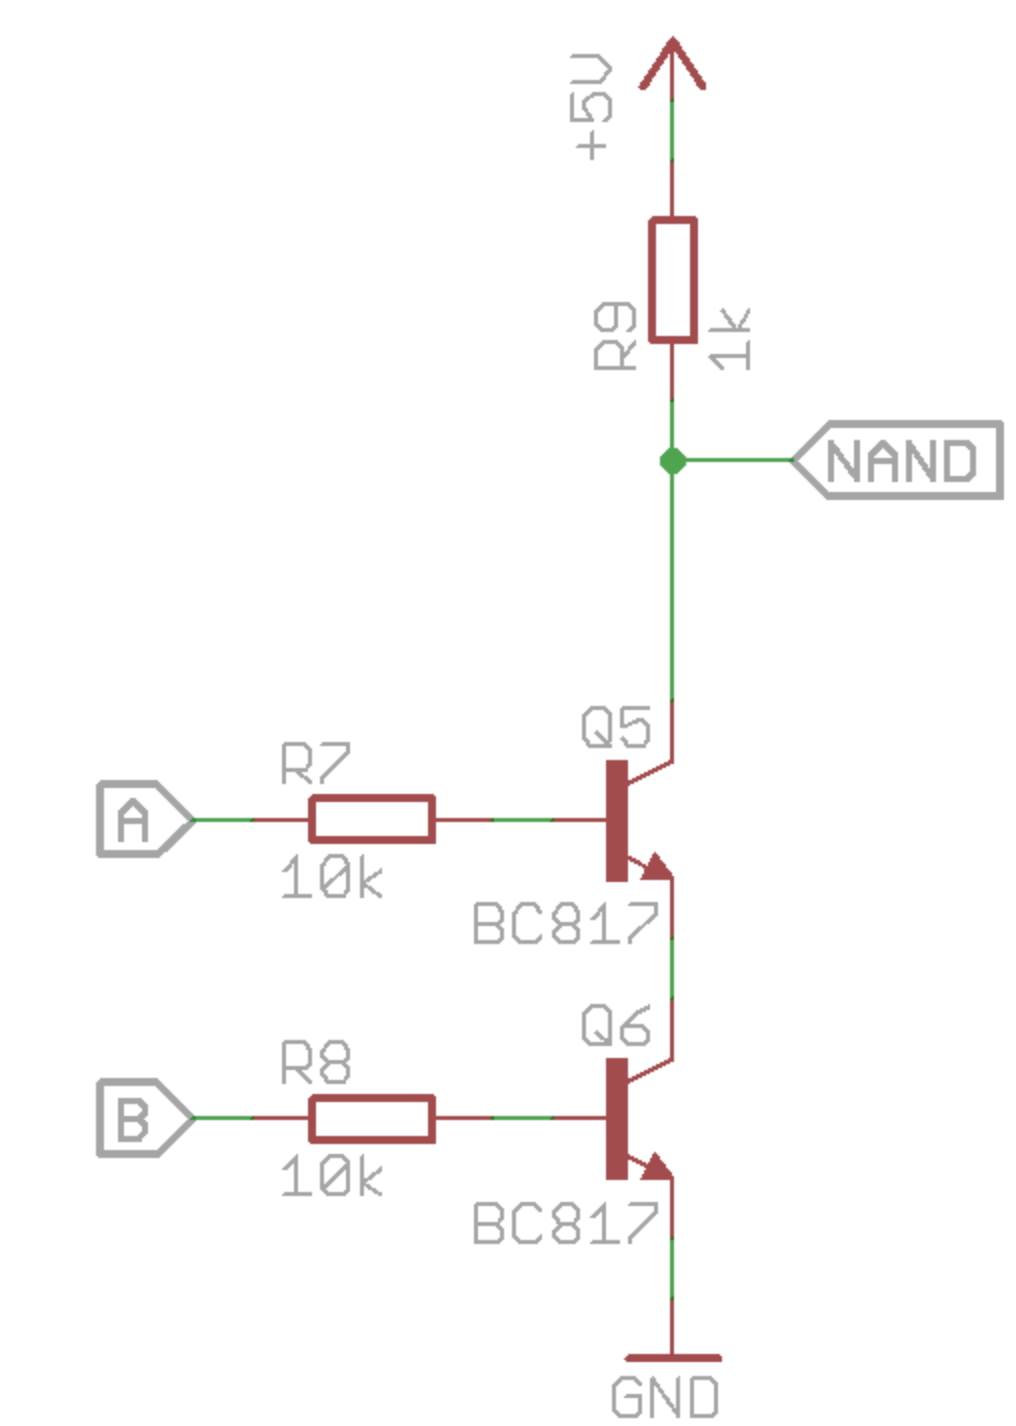
\includegraphics[width=0.35\textwidth]{figures/nand.png}
        }
        \href{https://project5474.org}{
            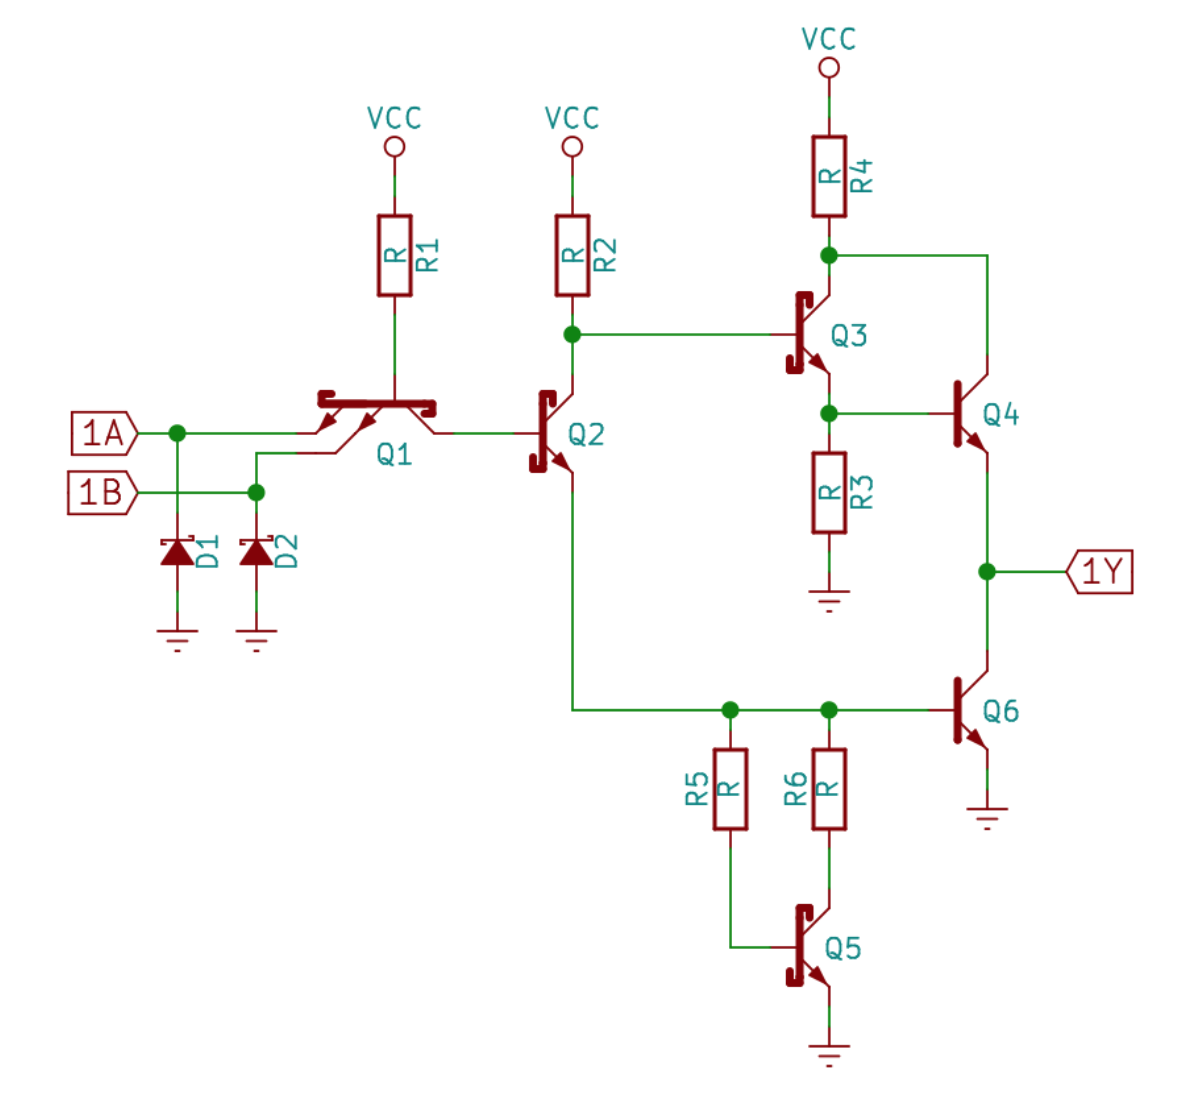
\includegraphics[width=0.5\textwidth]{figures/74LS00.png}
        }
        \caption{Implémentation naïve vs réèlle (74LS00) d'une porte NAND}
    \end{figure}

    Ainsi, seuls les diagrammes logiques de ces circuits intégrés seront considérés :

    \begin{figure}[ht!]
        \label{fig_nand_logic_diagram}
        \centering
        \href{http://www.ti.com/lit/ds/symlink/sn74ls00.pdf}{
        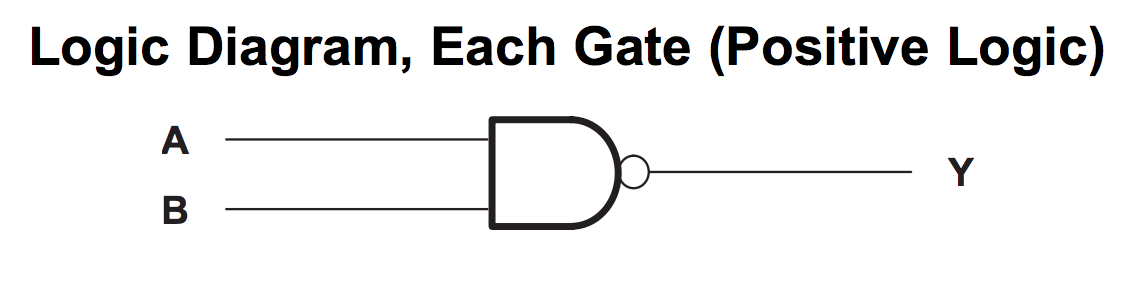
\includegraphics[width=0.5\textwidth]{figures/nand_logic_diagram.png}
        }
        \caption{Diagramme logique d'une NAND}
    \end{figure}

    Ce niveau d'abstraction permet de se focaliser sur le fonctionnement logique du processeur.
    La série de circuits intégrés 7400 de Texas Instruments sera utilisée car ceux-ci sont facilement
    trouvables, peu-chers et étaient très populaires durant l'age d'or des micro-ordinateurs.
    Plus précisément, nous utiliserons la sous-famille 74HCXX qui dispose d'une faible consommation
    énergétique grâce à la technologie CMOS et permet d'opérer à plusieurs MHz.
    Il faut toutefois faire attention à ne pas utiliser de composants de la sous-famille 74LSXX,
    très répendus mais qui utilisent des niveaux logiques incompatibles.

    \subsection{Phases de conception}

    \paragraph{}
    Le bon fonctionnement global du processeur ne pouvant être verifié qu'une fois les 9 modules
    achevés, il est préférable de simuler chaque module informatiquement dès le début de sorte à s'assurer
    qu'aucun problème d'ordre logique n'est présent dans l'implémentation proposée.  


    \subsubsection{Implémentation logique}

    \begin{figure}[ht!]
        \label{fig_ALU_logisim}
        \centering
        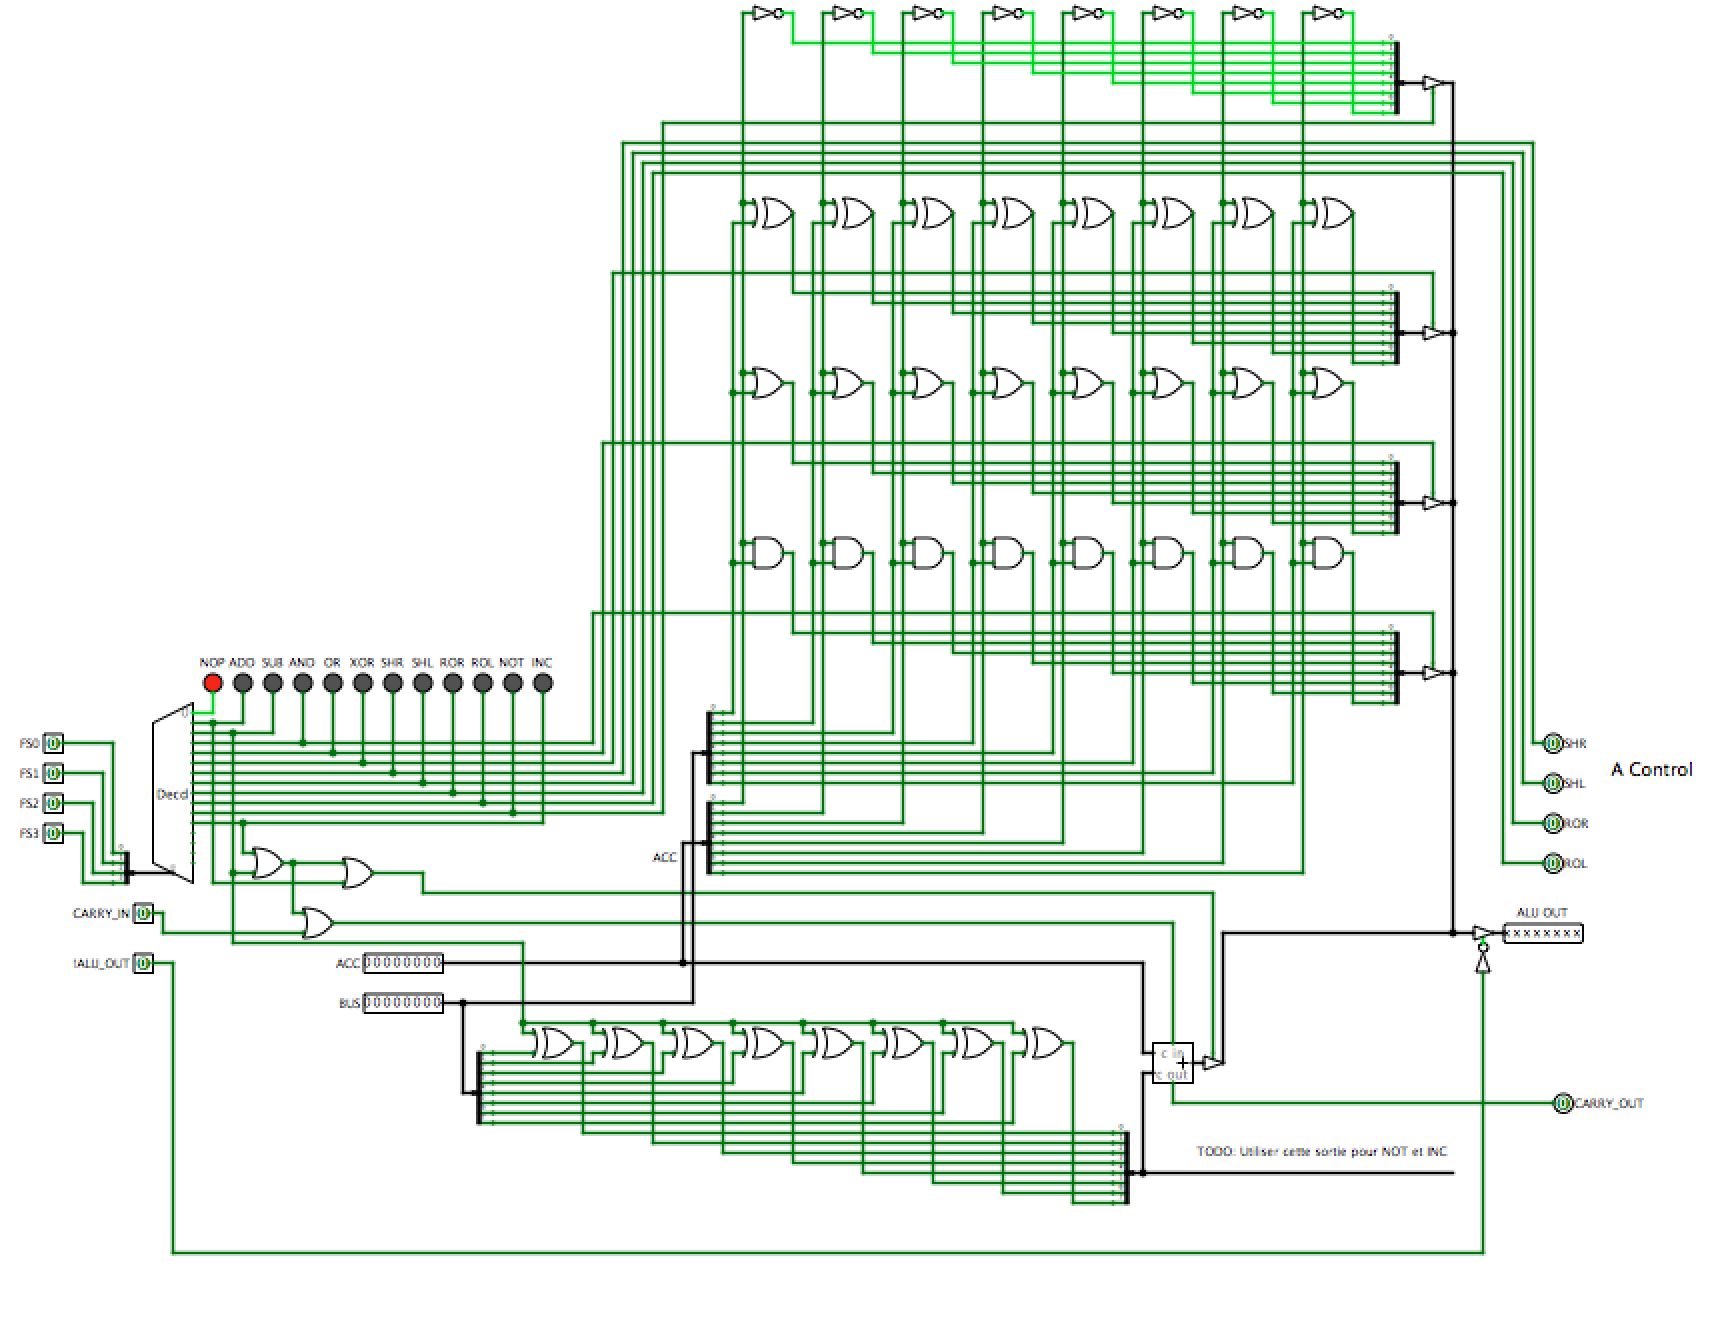
\includegraphics[width=0.5\textwidth]{figures/ALU_logisim.png}
        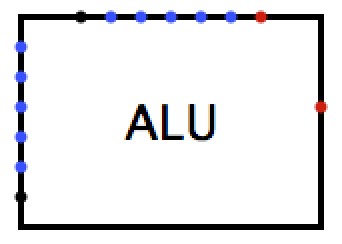
\includegraphics{figures/ALU_MOD.png}
        \caption{Module ALU simulé à l'aide de Logisim}
    \end{figure}

    Le logiciel de simulation de circuits logiques Logisim permet d'encapsuler un ensemble de portes
    logiques en un unique composant permettant ainsi d'integrer aisément plusieurs modules de façon lisible. 

    \subsubsection{Première implémentation physique}

    L'implémentation physique d'un module est plus complexe que la modelisation fonctionnelle, elle 
    contient notamment davantage d'éléments (condensateurs, resistances, boutons...).
    De plus, les fonctions logiques étant implémentées à l'aide de circuits intégrés, il est nécessaire 
    de s'assurer qu'ils soient branchés et utilisés correctement. Pour cela, une première implémentation 
    physique est réalisée sur des breadboard.

    \begin{figure}[ht!]
        \label{fig_CLK_breadboard}
        \centering
        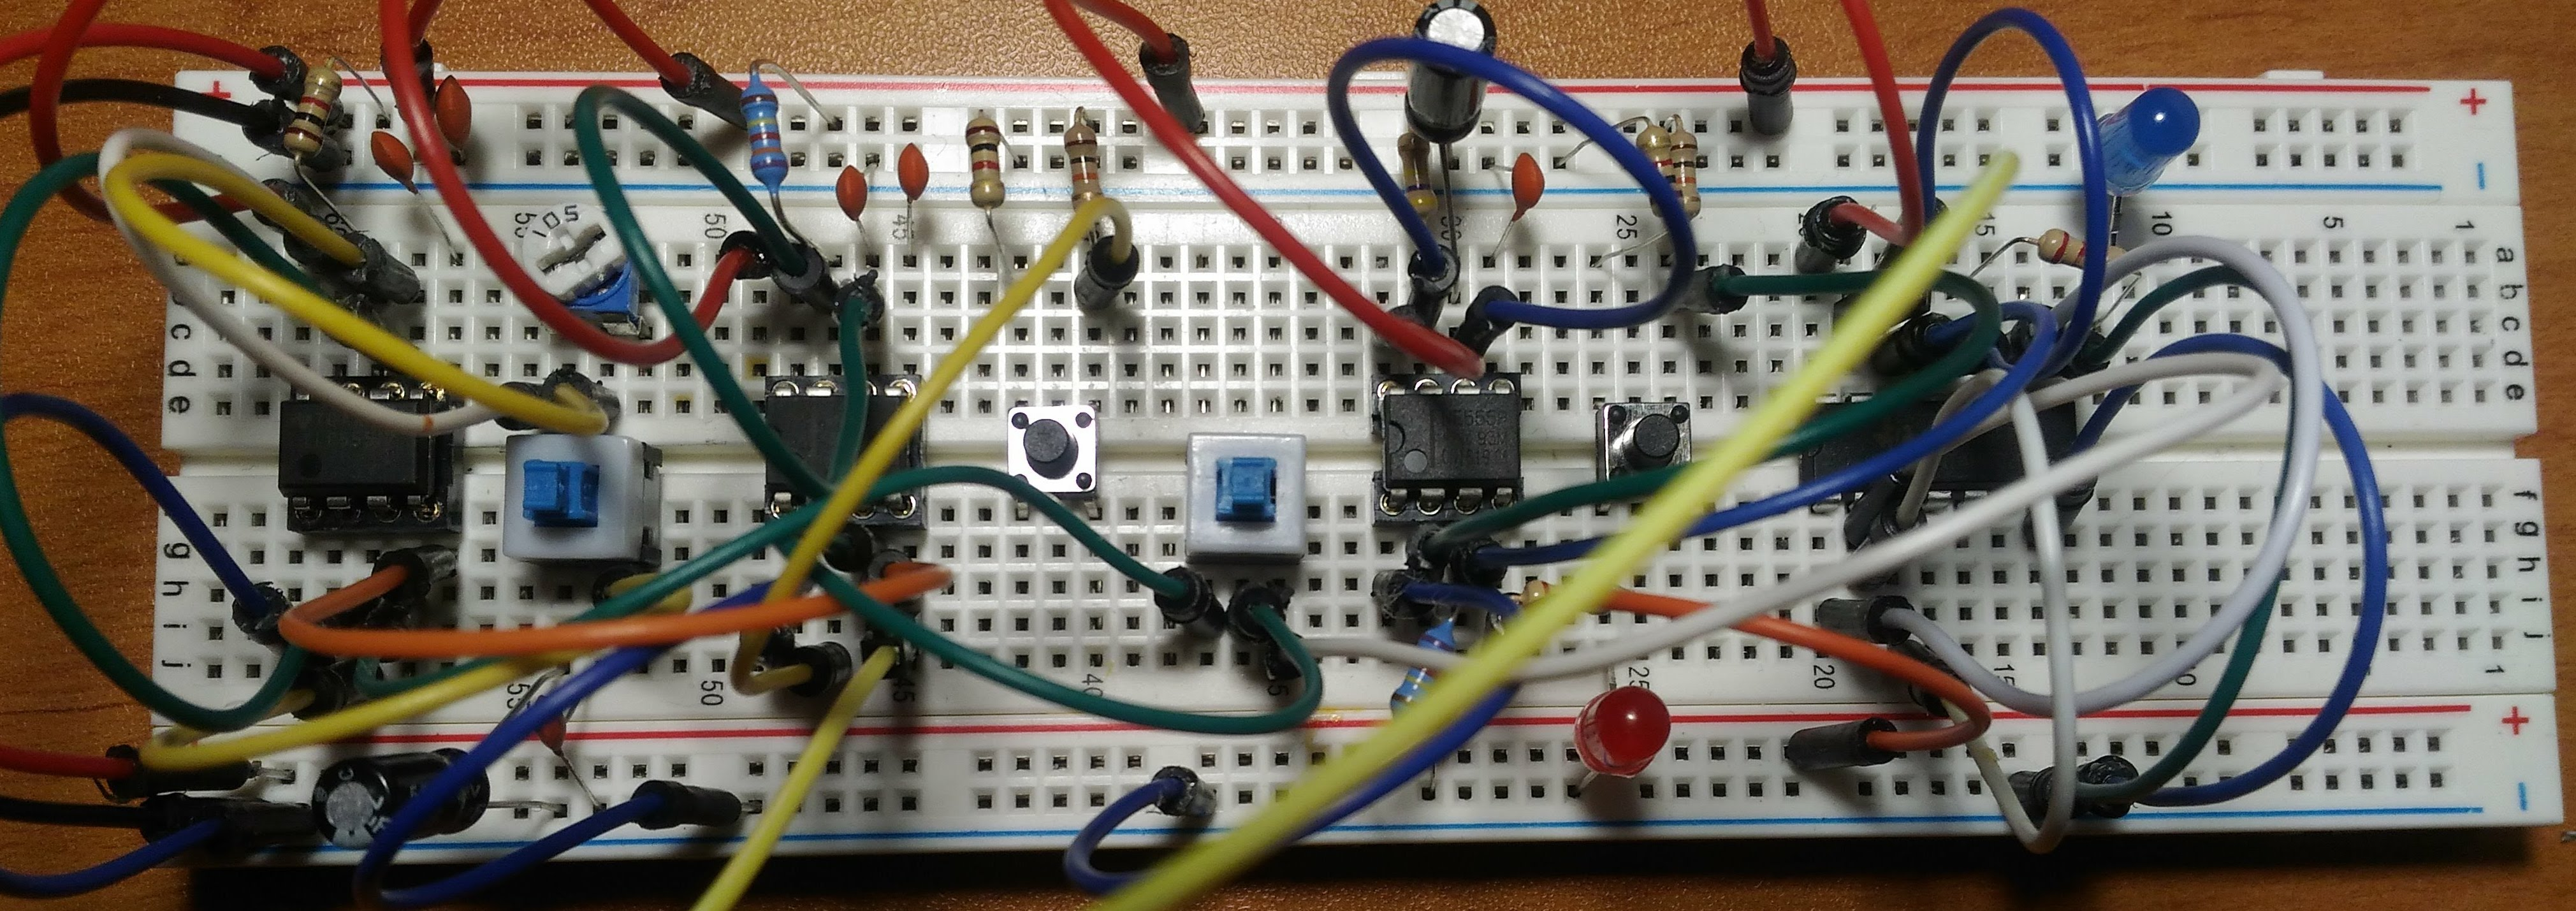
\includegraphics[width=\textwidth]{figures/CLK_breadboard.jpg}
        \caption{Module d'horloge et de reset implémenté sur une breadboard}
    \end{figure}

    \subsubsection{Conception du PCB}

    \begin{figure}[ht!]
        \label{fig_CLK_eagle}
        \centering
        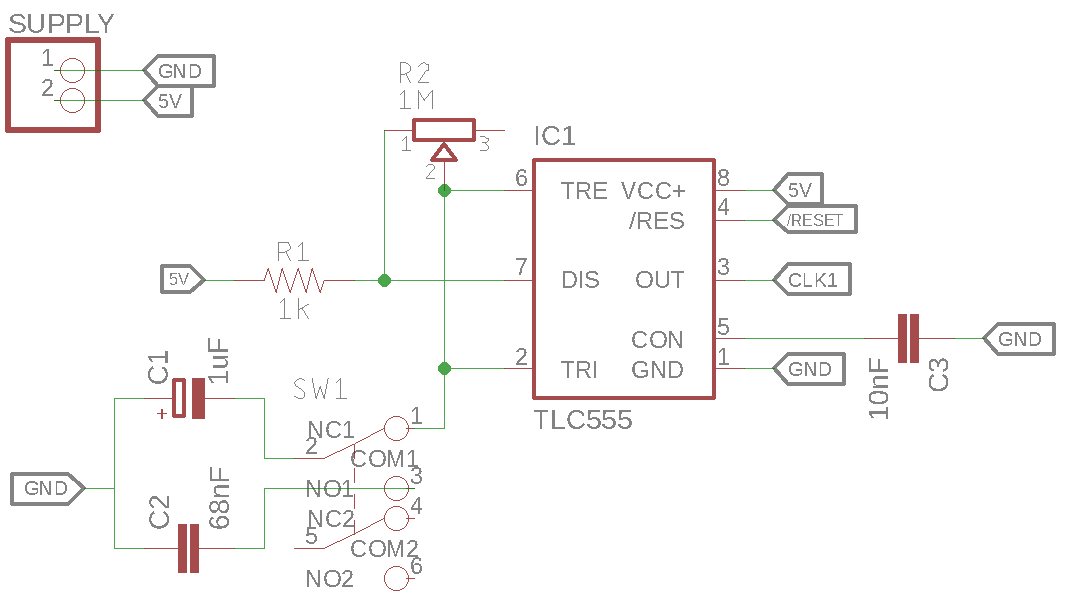
\includegraphics[width=\textwidth]{figures/CLK_eagle.png}
        \caption{Circuit de génération d'un signal carré de fréquence variable pour le module d'horloge}
    \end{figure}

    L'implémentation sur breadboard sert enfin comme référence pour les branchements
   lors de la réalisation des circuits sur Eagle.
   Une fois le routage effectué, un fichier gerberx est généré pour être lu par la graveuse à circuits
   de l'UTT, les composants et connecteurs sont ensuite soudés, des sockets DIP sont utilisés pour les 
   différents circuits intégrés afin de permettre leur utilisation sur une version ultérieure ou pour les
   changer en cas de non-fonctionnement.

   \newpage


   \section{Partie logicielle}

   La seconde partie du projet consiste à batir progressivement l'ensemble des programmes permettant
   une utilisation pratique de l'ordinateur, c'est à dire : \\

   \begin{itemize}
       \item Un système d'exploitation basique s'occupant d'initialiser les registres,
       ainsi que de gérer les interruptions
       \item Un assembleur réalisant la traduction d'instructions textuelles en binaire
       \item Un compilateur d'un subset restreint du langage C
   \end{itemize} 


\end{document}